\documentclass{F32}

\begin{document}
\begin{centering}
  \textbf{BACKGROUND AND GOALS FOR FELLOWSHIP TRAINING}\\
\end{centering}
%\textbf{Doctoral Dissertation and Prior Research Experience}\\
\subsubsection*{Doctoral Dissertation and Prior Research Experience}
%%%%%%%%%%%%%%%%%%%%%%%%%%%%%%%%%%%%%%%%%%%%%%%%%%%%%%%%%%%%%%%%%%%%%%%%%%%%%%%%
%Chemiluminescence
%\begin{wrapfigure}[24]{r}{8cm}
\begin{wrapfigure}{r}{8cm}
%\vspace{-0.2in}
\begin{centering}
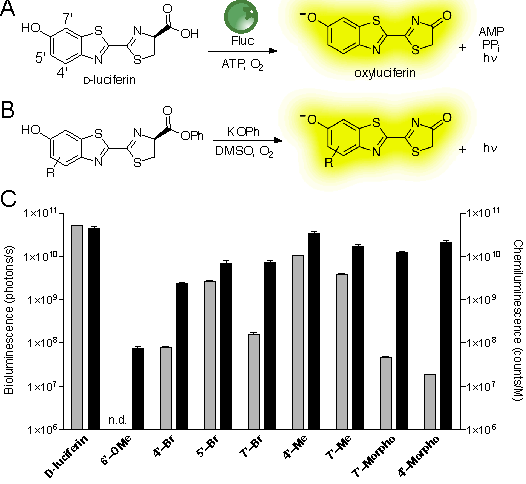
\includegraphics[width=\textwidth]{figures/previous_research/chemilum.pdf}

\end{centering}
\footnotesize
\caption{\label{figure:chemilum}
A) Oxidation of D-luciferin by firefly luciferase (Fluc) produces a photon of light. B) Luciferins can be activated and oxidized in a chemiluminescent manner to produce light. C) Comparison of bioluminescence (left axis, grey bars) and chemiluminescence (right axis, black bars) showed that many analogs were capable of robust light emission independent of enzyme.}
\end{wrapfigure}
%%%%%%%%%%%%%%%%%%%%%%%%%%%%%%%%%%%%%%%%%%%%%%%%%%%%%%%%%%%%%%%%%%%%%%%%%%%%%%%%
\textit{Graduate Research at the University California, Irvine, August 2012--May 2018. Supervised by Prof. Jennifer Prescher:}\\
Over the course of my graduate work I have developed the first example of multicomponent bioluminescence imaging with synthetic probes and gained broad experience in the areas of chemical biology and reaction methodology. These efforts combined my skills in chemical synthesis, biological assay development, and computer programming. My work has wide implications in the fields of imaging and protein engineering.

%\textbf{Expanding the imaging toolkit}\\
\subsubsection*{Expanding the imaging toolkit}
Genetically-encoded optical reporters have revolutionized our understanding of biological systems. These tools, namely fluorescent proteins, allow researchers to track multiple targets over extended periods of time in cellulo. However, the transition of fluorescent probes in vivo, to multicellular clinical models, has been hampered by the opacity of tissue and its propensity for autofluorescence. A complementary imaging technology, bioluminescence, does not suffer from these complications because it does not require excitation light (Rathbun, C. M. and Prescher, J. A. \textit{Biochemistry}, \textbf{2017}, \textit{56}, 5178.). Thus, the technique is exquisitely sensitive—with the ability to see as few as ten cells—and is often more suitable for imaging in thick tissues and entire organisms. Bioluminescence relies on luciferase enzymes that catalyze the oxidation of small-molecule substrates (luciferins), releasing photons of light in the process (Figure \ref{figure:chemilum}). Unfortunately, the optimal luciferases for in vivo use rely on the same small molecule luciferin, precluding studies of more than one feature or cell type at a time.

%%%%%%%%%%%%%%%%%%%%%%%%%%%%%%%%%%%%%%%%%%%%%%%%%%%%%%%%%%%%%%%%%%%%%%%%%%%%%%%%
%Parallel Screening
%\begin{wrapfigure}[21]{l}{8cm}
\begin{wrapfigure}{l}{8cm}
%\vspace{-0.2in}
\begin{centering}
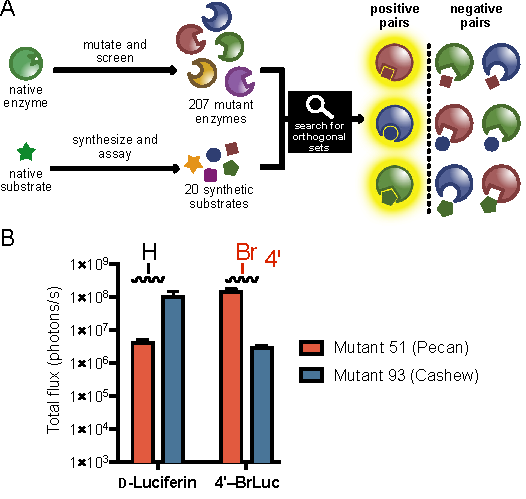
\includegraphics[width=\textwidth]{figures/previous_research/algorithmv2.pdf}
\end{centering}
\footnotesize
\caption{\label{figure:algorithm}
A) Strategy for developing orthogonal bioluminescent probes. A panel of luciferin analogs, and mutant luciferases are developed in parallel. A computer algorithm analyzes the dataset for orthogonal pairings. B) A top pair isolated via parallel screening. Luciferin-luciferase pairs reacted in a mutually exclusive manner.
}
\end{wrapfigure}
%%%%%%%%%%%%%%%%%%%%%%%%%%%%%%%%%%%%%%%%%%%%%%%%%%%%%%%%%%%%%%%%%%%%%%%%%%%%%%%%

To address this issue, I developed and analyzed a number of new luciferin probes, and created a selection platform to find mutually orthogonal luciferases and luciferins for multicomponent imaging. In contrast to the spectroscopic resolution of fluorescent tools, these probes were designed to exhibit substrate resolution. Since red light is the only color capable of penetrating tissue, spectral resolution in vivo is difficult to achieve. Thus, I resolved to take advantage of the molecular component of bioluminescence imaging to develop exclusively selective luciferin-luciferase pairs.

\textit{Brominated luciferins are versatile bioluminescent probes}\\
My strategy for mutually selective probes relied on synthesizing small molecule luciferin analogs and screening them against libraries of functional mutant luciferases. I initially focused on development of minimally perturbed luciferin probes. We rationalized that bromination of the luciferin core might perturb binding to the wildtype enzyme, yet retain inherent light-emitting ability of the molecule. Directed evolution could then be used to restore light emission. To verify this, I developed a chemiluminescence assay to test the relative light-emitting abilities of our luciferin analogs (Figure 1B). Gratifyingly, the brominated probes showed robust emission, indicating that these molecules had the potential to be capable emitters (Figure 1C). Additionally, I have shown that cross-coupling reactions can be used to derivatize the brominated luciferins, producing a variety of modified scaffolds in a divergent manner. This work resulted in a publication in ChemBioChem (Steinhardt, R. C. \textit{et al.}, \textit{ChemBioChem}, \textbf{2016}, \textit{18}, 96.). In addition to the brominated variants, my colleagues and I synthesized a wide variety of modified luciferins analogs—ranging from subtle electronic modifications, to large steric perturbations. The chemiluminescence assay has proven general for these analogs as well, providing a benchmark for light emission before mutant luciferases are developed.

%%%%%%%%%%%%%%%%%%%%%%%%%%%%%%%%%%%%%%%%%%%%%%%%%%%%%%%%%%%%%%%%%%%%%%%%%%%%%%%%
%\begin{wrapfigure}[25]{r}{7cm}
\begin{wrapfigure}{R}{7cm}
%\vspace{-0.2in}
\begin{centering}
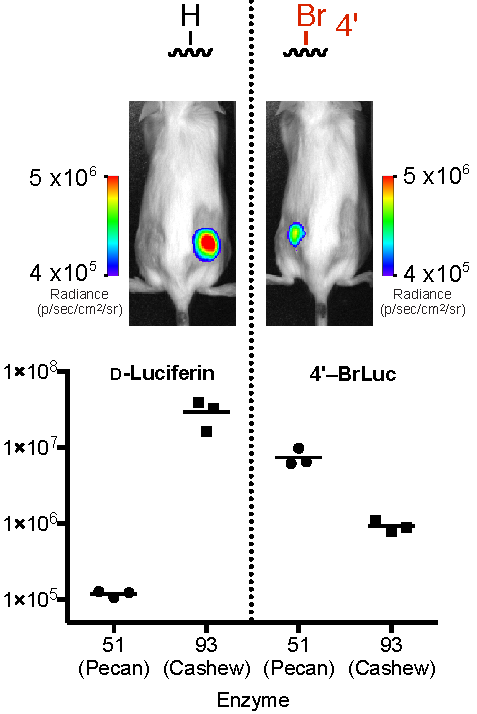
\includegraphics[width=\textwidth]{figures/previous_research/mouse1pc.pdf}

\end{centering}
\footnotesize
\caption{\label{figure:mice}
Mutually orthogonal pairs enable multicomponent imaging in mouse models, however, the images acquired above were taken 8-12 hours apart to allow dissipation of prior signal.
}
\end{wrapfigure}
%%%%%%%%%%%%%%%%%%%%%%%%%%%%%%%%%%%%%%%%%%%%%%%%%%%%%%%%%%%%%%%%%%%%%%%%%%%%%%%%

\textit{Orthogonal Luciferase-luciferin pairs for bioluminescence imaging}\\
Next, we sought to identify luciferase mutants that selectively utilized our luciferin analogs. We designed and generated a range of functional luciferases that reflected a variety of mutations about the active site. Combining molecules and enzymes, we tested 20 luciferins with 207 mutant luciferases (Figure \ref{figure:algorithm}). The screening experiment generated 4,140 enzyme-substrate combinations, and thus a potential for more than 4 million possible sets of two substrates and two enzymes. Since it would be impractical to evaluate all of these combinations manually, I first derived a mathematical quantification of orthogonality to ‘score’ each potential pairing. Next, I wrote a supercomputer algorithm to search this dataset in a matter of minutes for the highest-scoring pairs. The software provided a ranked list of mutually orthogonal enzyme-substrate pairs that were biochemically verified. A top hit from this list is shown in Figure \ref{figure:algorithm}B. Each enzyme exhibited greater than ten-fold preference for its matched substrate. Resolution was maintained when these probes were moved into mouse models, highlighting the speed and accuracy of our approach (Figure 3A). As a next step, I have been searching the data sets for not just pairs of bioluminescent tools, but triplet and quadruplet sets of orthogonal probes. This would enable visualization of three or more populations of interest simultaneously. However, the problem becomes much more complex due to the increase in possible pairings (Figure \ref{figure:algorithm}A). Using my algorithm, I have identified 6,171 possible sets of orthogonal triplets, several of which have been verified in bacterial lysate. This work resulted in publications in JACS, and ACS Central Science (Rathbun, C. M. \textit{et al.}, \textit{J. Am. Chem. Soc.}, \textbf{2017}, \textit{139}, 2351. and Rathbun, C. M. \textit{et al.}, \textit{ACS Cent. Sci.}, \textbf{2017}, \textit{3}, 1254.). We hope to use these tools to monitor the locations of cancer cells and the immune system throughout disease progression. Collectively, our orthogonal pairs will enable a variety of multicomponent, in vivo imaging studies, and my screening techniques and computer algorithm will enable advances in other areas of chemical biology.

%%%%%%%%%%%%%%%%%%%%%%%%%%%%%%%%%%%%%%%%%%%%%%%%%%%%%%%%%%%%%%%%%%%%%%%%%%%%%%%%
%Unmixing in vivo
%\begin{wrapfigure}[15]{l}{11cm}
\begin{wrapfigure}{L}{10cm}
%\vspace{-0.2in}
\begin{centering}
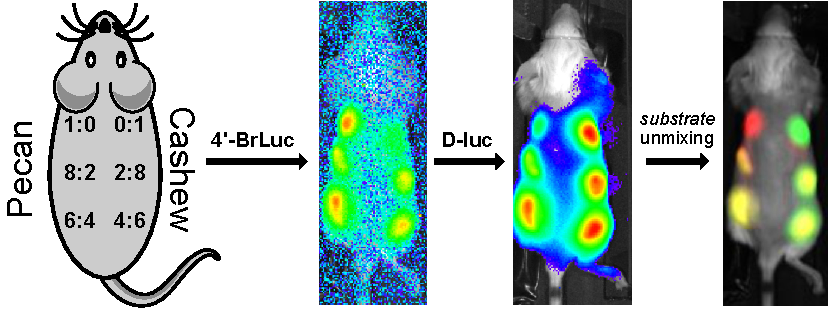
\includegraphics[width=\textwidth]{figures/previous_research/mouse_unmixing.pdf}

\end{centering}
\footnotesize
\caption{\label{figure:mouse_unmixing}
Mixtures of cell populations can be distinguished in a live mouse. Tumors containing varying amounts of cells expressing Pecan and Cashew were implanted into the back of live mice. Substrates were injected i.p. in a sequential fashion, and images were taken between each injection.
}
\end{wrapfigure}
%%%%%%%%%%%%%%%%%%%%%%%%%%%%%%%%%%%%%%%%%%%%%%%%%%%%%%%%%%%%%%%%%%%%%%%%%%%%%%%%

\textit{Expanding the scope of multicomponent imaging}\\
My most recent work focused on increasing the practicality of these tools for preclinical in vivo imaging. The major drawbacks of our substrate resolution approach included temporal resolution and background emission. I addressed these issues by utilizing traditional spectral unmixing algorithms to deconvolute substrate signals mathematically. This enabled sequential imaging of substrates, and the ability to resolve smaller numbers of cells. With a top orthogonal pair we ``unmixed" gradients of mutant luciferases in bacterial lysate and resolved mixtures of these mutants in mouse tumor models. Tumors were implanted in mice with varying mixtures of mammalian cells expressing our top probes. Luciferin substrates were sequentially administered and images were acquired between injections. The images were then ``unmixed" and overlayed (Figure \ref{figure:mouse_unmixing}). The lab is currently applying these techniques to track cells involved in metastasis \textit{in vivo}.

%\textbf{Previous work in transition metal catalysis methodology}\\ % QUESTION keep this section here??
\subsubsection*{Previous work in transition metal catalysis methodology}
I spent the first year and a half of my graduate work in the lab of Professor Vy Dong. During this time, I sought new, streamlined methods of carbohydrate synthesis. We developed a new method of selectively acylating sugars via copper catalysis (Chen, I. H. \textit{et al.}, \textit{Chem. Eur. J.}, \textbf{2014}, \textit{20}, 5013.). Our catalysts could distinguish between three similar alcohols moieties to acylate at a set position, depending on the ligand used. This method proved general for a variety of sugar scaffolds containing cis diols.

%\textbf{Goals for Fellowship Training}\\
\subsubsection*{Goals for Fellowship Training}
My ultimate career goal is to obtain a professorship at an R01 institution. I envision a research program at the interface of organic chemistry and protein engineering. Parallel modification of enzymes and their substrates was a cornerstone of my graduate work. And a large aspect of my postdoctoral studies will involve the effects of modifying a ligand and its natural RNA riboswitch. Such studies, and the effect that they have on selectivity, will continue into my independent career. In addition to leading innovative research, I look forward to mentoring new scientists within my lab, at the undergraduate, graduate, and postdoctoral levels. Additionally, a professorship provides a platform for communication of science to the public in an approachable way.

Thus far my scientific training has placed me at a unique position between organic chemistry and chemical biology. During my undergraduate studies at Hope College, I conducted rigorous physical organic studies of reaction mechanisms. While in the Dong lab at UC Irvine, I leveraged these skills to develop new metal-catalyzed organic transformations. Upon my transition to the Prescher lab, my training in organic chemistry allowed me to think deeply about enzyme catalysis, and the factors that effect binding and turnover. As I continue on to the Palmer lab, this funding will enable me to gain additional training in the study of biological systems on the cellular level. As I continue to hone my skills in organic chemistry and biomolecule engineering, I will learn new skills in microscopy and cell culture. With a diverse mentoring team (Pamer, Rinn, and Batey), I will be exposed to all aspects of tool development on a cellular level.

%The unique focus on RNA in the Biofrontiers Institute at CU Boulder will also enable me to initiate interdisciplinary collaborations...

I also intend to use my time as a postdoc to gain additional ``soft'' skills. This funding will give me the freedom to mentor undergraduate and graduate students in the Palmer lab; a crucial skill for my future as a professor. Additionally, I intend to present my work at a venues such as Gordon conferences, Cold Spring Harbor Labs, and EMBL conferences, and continue to build my network with other researchers in the field. With respect to teaching, I am excited to attend the New Assistant Professor Program offered by the Faculty Teaching Excellence Program at CU Boulder. This program helps postdocs and pre-tenure faculty gain the tools and skills that they need to become engaging and informative in the classroom. Professor Palmer is very supportive of these pursuits, and will offer advise with respect to additional training opportunities that I should pursue.

%\textbf{Activities Planned Under this Award}\\
\subsubsection*{Activities Planned Under this Award}
If received, I will spend the majority of my time in pursuit of the described aims. Syntheses of relevant molecules will be carried out, and data acquisition and relevant experiments will be performed. Additionally, time will be spent in preparation of written and oral communications of important results of the project in the form of publications, posters, and oral presentations and seminars (65\%).
A portion of my time will also be spent mentoring undergraduate and graduate students in the Palmer lab. This will be a crucial activity, as my final career goal is to become a professor at a research institution. I'll also meet with Professor Palmer regularly to discuss mentorship and the best practices thereof (15\%).
To stay up-to-date on the important research being conducted at CU Boulder and across the country, I will attend a variety of scientific seminars in a range of disciplines. The Palmer lab is involved in supergroups within Biophysics, Signaling and Cellular Regulation, Chemical Biology, RNA, and Bioinformatics. These talks give CU Boulder researchers a chance to hear about work going on around them, and enables crosstalk and collaborations (5\%).
In addition to the Responsible Conduct of Research class offered at CU Boulder, I will also pursue opportunities to receive additional training in data science and bioinformatics. Professor Palmer has also recommended that I attend the intensive workshop provided by Cold Spring Harbor Lab called ``Quantitative Imaging: From Acquisition to Analysis'' (5\%).
To interact with other scientist from around the world, and present my relevant research results, I plan to attend conferences hosted by (but not limited to) the American Chemical Society and the Gordon Research Conferences (5\%).
The New Assistant Professor Program offered by the Faculty Teaching Excellence Program at CU Boulder will help me gain soft skills necessary for being an effective professor in the future (5\%).

For Years 2 and 3, I will focus more on preparations for my independent career, shifting my tasks accordingly:

\subsubsection*{Year 2:}
Research (65\%), Mentoring students (10\%), Seminars (5\%), Scientific Training (5\%), Conferences (5\%), soft skills training (5\%), Developing independent research ideas (5\%)

\subsubsection*{Year 3:}
Research (50\%), Mentoring students (10\%), Seminars (5\%), Scientific Training (5\%), Conferences (5\%), soft skills training (5\%), Developing independent research ideas (5\%), Networking (5\%), Applying for tenure-track positions (10\%).

\end{document}
